\subsection{Verifica della documentazione}
	Per la verifica della documentazione si utilizza la tecnica del \glock{walkthrough} revisionando i documenti per intero e la tecnica di \glock{inspection}.

\subsubsection{Calcolo leggibilità e controllo ortografia dei documenti}
	Per verificare quanto sono leggibili i documenti redatti si utilizza l'\glock{indice di gulpease} ed è stato effettuato un controllo di ortografia. La seguente tabella contiene i risultati ottenuti ad ogni release dei documenti:

\begin{table} [h!]
	\rowcolors{2}{gray!25}{gray!6}
	\begin{center}
		\begin{tabular} { c c c c}
			\rowcolor{lightgray}
			\textbf{Documento}&\textbf{Errori ortografici}&\textbf{Indice di gulpease}&\textbf{Esito}\\
			\dext{Piano di progetto v1.0.0}		& 0 & 59  &Superato\\
			\dext{Norme di progetto v1.0.0} 	& 0	& 64  &Superato\\
			\dext{Studio di fattibilità v1.0.0}	& 0	& 57  &Superato\\
			\dext{Glossario v1.0.0}				& 0	& 47  &Superato\\
			\dext{Piano di qualifica v1.0.0}	& 0	& 48  &Superato\\
			\dext{Media verbali v1.0.0}			& 0	& 68  &Superato\\
			\dext{Analisi dei requisiti v1.0.0}	& 0	& 72  &Superato\\
            \dext{Piano di progetto v2.0.0}		& 0 & XX  &Superato\\
            \dext{Norme di progetto v2.0.0} 	& 0	& XX  &Superato\\
            \dext{Studio di fattibilità v2.0.0}	& 0	& XX  &Superato\\
            \dext{Glossario v2.0.0}				& 0	& XX  &Superato\\
            \dext{Piano di qualifica v2.0.0}	& 0	& XX  &Superato\\
            \dext{Media verbali v2.0.0}			& 0	& XX  &Superato\\
            \dext{Analisi dei requisiti v2.0.0}	& 0	& XX  &Superato\\
		\end{tabular}
	\end{center}
	\caption{Esiti verifiche automatizzate - Revisione di Progettazione}
\end{table}

\noindent Con i seguenti grafici, illustriamo l'andamento dell'indice di gulpease e degli errori ortografici riscontrati per ogni documento, nelle revisioni effettuate:
\begin{figure}[H]
	\centering
	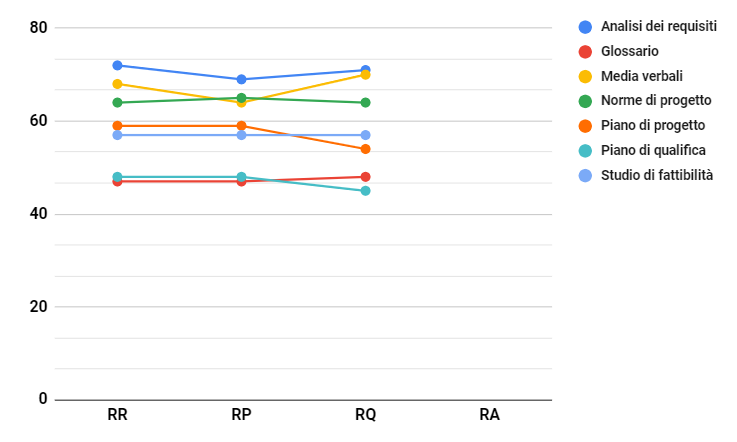
\includegraphics[width=12cm]{images/gulpease.png}
	\caption{Indice di gulpease per revisione}
\end{figure}
\begin{figure}[H]
	\centering
	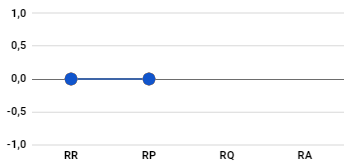
\includegraphics[width=9cm]{images/err_ortografici.png}
	\caption{Errori ortografici per revisione}
\end{figure}

\subsection{MP06 - Budget variance}
La seguente metrica verrà tracciata per verificare se si è speso di più o di meno rispetto a quanto previsto.
%\begin{figure}[H]
%	\centering
%	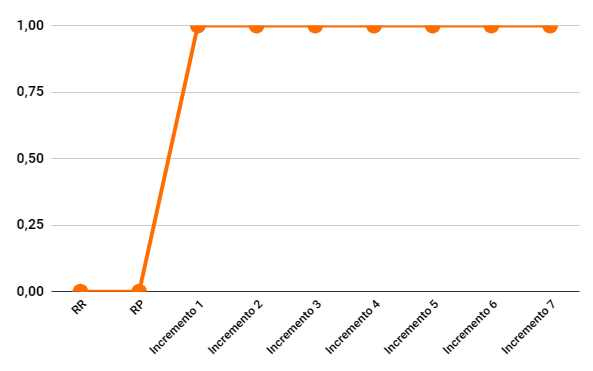
\includegraphics[width=9cm]{images/unbudgeted_risks.png}
%	\caption{Andamento metrica budget variance}
%\end{figure}

\subsection{MP07 - Unbudgeted risks}
Data la possibilità di incontrare rischi, non preventivati in fase di analisi, di seguito verranno illustrate tali evenienze per ogni revisione del progetto:
\begin{figure}[H]
	\centering
	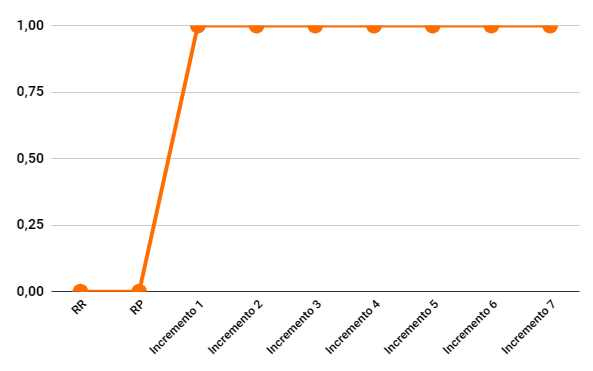
\includegraphics[width=12cm]{images/unbudgeted_risks.png}
	\caption{Andamento metrica unbudgeted risks}
\end{figure}

